\documentclass[11pt,a4paper, twocolumn]{article}

\usepackage{acl2020}

\usepackage{times}
\usepackage{latexsym}

\usepackage{graphicx}
\graphicspath{ {./img/} }

\renewcommand{\UrlFont}{\ttfamily\small}

% This is not strictly necessary, and may be commented out,
% but it will improve the layout of the manuscript,
% and will typically save some space.
\usepackage{microtype}

\aclfinalcopy % Uncomment this line for the final submission
%\def\aclpaperid{***} %  Enter the acl Paper ID here

%\setlength\titlebox{5cm}
% You can expand the titlebox if you need extra space
% to show all the authors. Please do not make the titlebox
% smaller than 5cm (the original size); we will check this
% in the camera-ready version and ask you to change it back.

\title{Disability Trends: An examination of global disability-related terminology}

\author{Noah Duggan Erickson \\
  Dept. of Computer Science \\
  Western WA University \\
  Bellingham, WA, USA \\
  \texttt{email@redacted.com} \\\And
  Brady Deyak \\
  Dept. of Computer Science \\
  Western WA University \\
  Bellingham, WA, USA \\
  \texttt{email@redacted.com} \\\And
  Raghav Vivek \\
  Dept. of Computer Science \\
  Western WA University \\
  Bellingham, WA, USA \\
  \texttt{email@redacted.com} \\}

\date{10 June 2024}

\begin{document}
\maketitle
\begin{abstract}
This document contains the instructions for preparing a manuscript for the proceedings of ACL 2020.
The document itself conforms to its own specifications, and is therefore an example of what your manuscript should look like.
These instructions should be used for both papers submitted for review and for final versions of accepted papers.
Authors are asked to conform to all the directions reported in this document.
\end{abstract}

\section{Introduction}
Intro text goes here.

\section{Related Work}
Related work goes here.

\section{Our Approach}
Despite the highly multidisciplinary nature of the project, the present work is primarily focused on the natural language processing aspect. The project was divided into three main parts: data acquisition and pre-processing, word vectorization, and sentiment analysis. The data acquisition and pre-processing part of the project involved scraping a large number of news articles from Nexis Uni, converting them to plaintext, and then lemmatizing the text. The word vectorization part of the project involved training a FastText model on the lemmatized text and then visualizing the results. The sentiment analysis part of the project involved training a sentiment analysis model on the lemmatized text and then interpreting the results. The project was conducted using Python and multiple libraries, including \texttt{Stanza}~\citep{stanza}, \texttt{Gensim}~\citep{gensim}, \texttt{TensorFlow}~\citep{tensorflow}, and \texttt{Alibi}~\citep{alibi}.

\section{Experiments}
There were multiple experiments run throughout the project. These include a massive scraping operation with subsequently large-scale data pre-processing, a word vectorization model, and an interpretable sentiment analysis model.

\subsection{Data Sources}

The data for this project was acquired using the export feature of Nexis Uni. Using this feature, a large number of news articles were downloaded as rtf files. These were then converted to plaintext using the \texttt{striprtf}~\citep{striprtf} Python library. Each article's content was then preprocessed using the lemmatization pipeline in the \texttt{Stanza}~\citep{stanza} library. This pipeline tokenizes the text, removes stopwords, and lemmatizes the remaining words using a neural seq2seq model. The resulting data was then stored as a list and exported to JSON alongside article metadata.

\subsection{Word Vectorization}

The word vectorization model used was the FastText model from the \texttt{Gensim} library. After training the model on the preprocessed data from a given decade, the model was used to generate a list of the most similar words to a list of selected words. The results were then visualized using a t-SNE plot. The t-SNE plot was generated using the \texttt{Plotly} library.

\subsection{Word Cloud}

Another such visual representation of the data after pre-processing was a word cloud generated using the \texttt{WordCloud} library and \texttt{matplotlib}. The word cloud was then generated using word frequencies to set the size of each word.

\subsection{Sentiment Analysis}
\textbf{BRADY}: In this part of the project, we used the Valence Aware Dictionary and sEntiment Reasoner or \textbf{VADER} and the LSTM model of TensorFlow Keras, a machine learning tool created by Google to generate and visualize data flow. In this case, we used TensorFlow Keras to train a sentiment analysis model similar to the one proposed in this paper. Once the sentiment scores for each document are calculated and the model is built, the data is trained and fit to the model. The average accuracy of this model was shown to be $82.5$\%. For the 2010s decade, we took this model and then used it to predict from the training data the sentiment of the entire decade. The result was that the overall sentiment of disability in the 2010s was positive. We plan to continue building upon the sentiment analysis model and having TensorFlow be able to cover all the decades and their sentiment.

\subsection{Interpretable Sentiment Analysis}
We chose the Alibi library and the integrated gradients method to create interpretations. Integrated grardietns define and attribution value foro each word in the input. Attributions are calcuclated using the integral of hte model gradients with respect ot he word embedding layer along a straight path from a base line instance to the input instance. To do othis, we take the model, a sambple of the data, and an index of words to compare frequencies and setiment against. We use this to create a visualization. The visualiation is based on the what has the highest positive attribution. Words with high positive attribution are highlighted in shades of green and words with negative attributions in shades of pink. Positive attributions can be interpreted as increase in probability of the predicted class (``positive sentiment'') while negative attributions correspond to decrease probability of the predicted class.

\section{Results}
Multiple visualizations and analyses were conducted on the data. These include a word vectorization model, a document-level sentiment analysis model, and an explanation of said sentiment analysis model.

\subsection{Word Vectorization}

Word vectorization models were trained on the data for each search term for each decade. This allows for the visualization of not only the most similar words to a given word in that snapshot, but also how the clusters of words shift over time. For example, figures \ref{tsnea} and \ref{tsneb} show the tsne plots for selected words using the ``disab'' search term from the 1990s and 2020s, respectively.

\begin{figure}
  \centering
  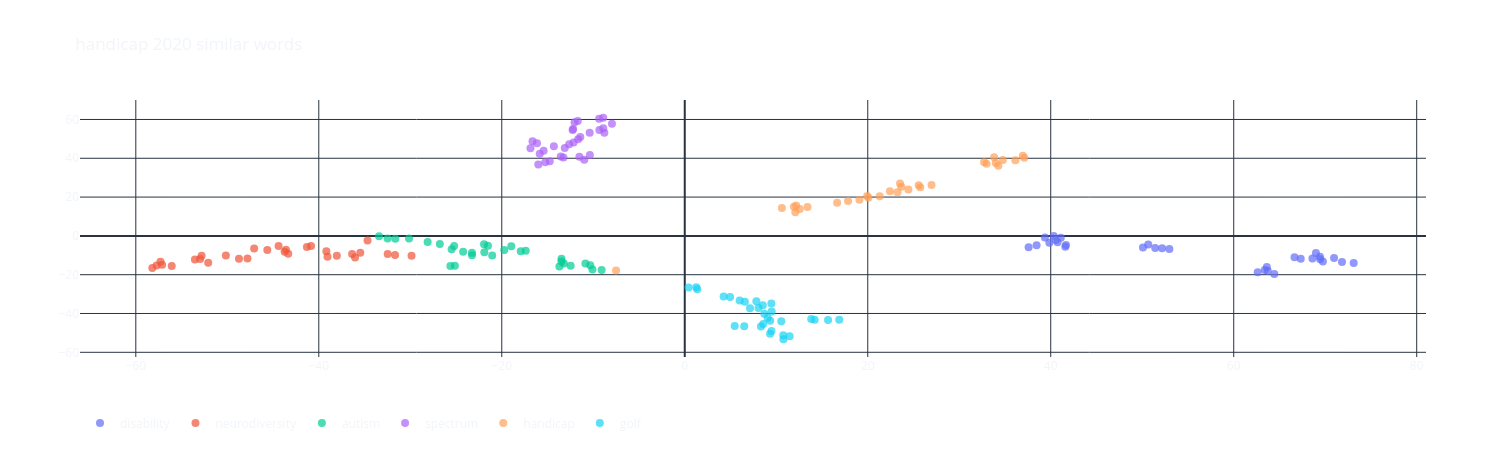
\includegraphics[width=0.5\textwidth]{lemma_disab_1990_simword.png}
  \caption{\label{tsnea} t-SNE plot of the word vectorization model using the ``disab'' search term from the 1990s.}
  
\end{figure}
  
\begin{figure}
  \centering
  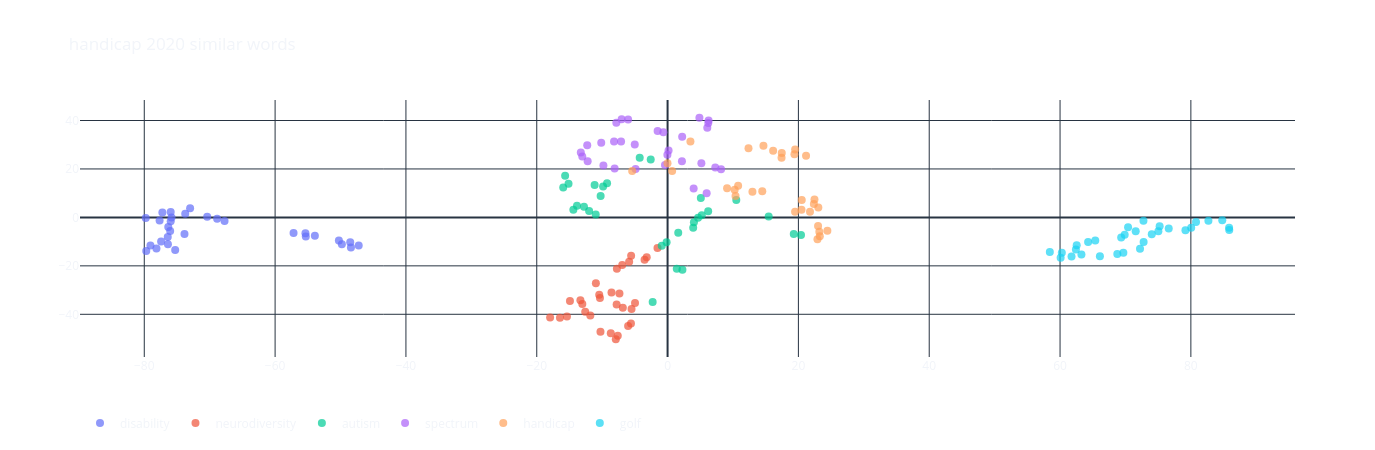
\includegraphics[width=0.5\textwidth]{lemma_disab_2020_simword.png}
  \caption{\label{tsneb} t-SNE plot of the word vectorization model using the ``disab'' search term from the 2020s.}
  
\end{figure}

\subsection{Word Cloud}

Word clouds for each term and decade were generated using the word frequencies from the pre-processed data. These word clouds give a visual representation of the most common words in the data. For example, figures \ref{wca} and \ref{wcb} shows the word cloud for the ``disab'' search term from the 1990s and 2020s.

\begin{figure}
  \centering
  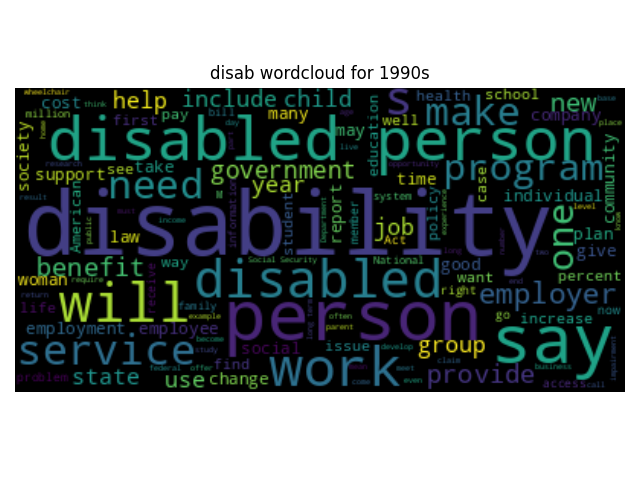
\includegraphics[width=0.5\textwidth]{lemma_disab_1990_wordcloud.png}
  \caption{\label{wca} Word cloud of the word frequencies for the ``disab'' search term from the 1990s.}
\end{figure}

\begin{figure}
  \centering
  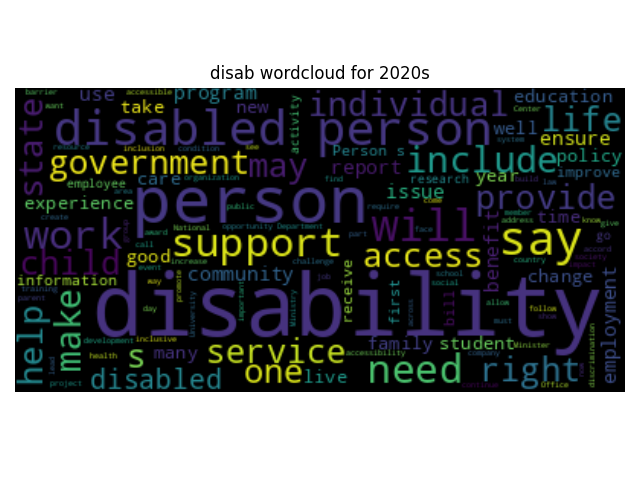
\includegraphics[width=0.5\textwidth]{lemma_disab_2020_wordcloud.png}
  \caption{\label{wcb} Word cloud of the word frequencies for the ``disab'' search term from the 2020s.}
\end{figure}

\section{Discussion}
As alluded to in our approach, the goal of this project was to create a tool that can be used by other researchers to conduct analyses on disability-related terminology and beyond. As such, the discussion of specific points of interest is outside the scope of this project. However, the results of the analyses shown above represent just the tip of the iceberg of what can be done with this data and these models. The word vectorization model, for example, can be used to track the evolution of disability-related terminology over time. The sentiment analysis model can be used to track the sentiment of news articles over time. The word cloud can be used to track the most common words in news articles over time. The possibilities are endless.

Furthermore, despite the name of this project, the general idea can be easily extended into other areas simply by using different search terms. For example, one could use the same pipeline to track the evolution of sentiment towards mass transit and transit-oriented development. 

\section{Conclusion}
Due to the short turn-around time of the project, avenues for future work are plentiful. These include a more centralized system for creating the analyses, a more robust sentiment analysis model, and a deeper review of these analyses from a critical disability studies and sociological perspective.

\bibliography{report}
\bibliographystyle{acl_natbib}

\end{document}
